\documentclass[11pt,a4paper]{article}
\usepackage[margin=2.2cm]{geometry}
\usepackage{amsmath,amssymb,xcolor,enumitem,booktabs,graphicx,longtable}
\usepackage[normalem]{ulem}
\setlength{\parskip}{0.6em}\setlength{\parindent}{0pt}
\definecolor{newc}{HTML}{1f6f43}
\newcommand{\new}[1]{\textcolor{newc}{#1}}
\newcommand{\old}[1]{\textcolor{gray}{\sout{#1}}}
\newcommand{\note}[1]{{\small\itshape [#1]}}
% Labels print as their names, so the text can be pasted back as it stands.
\newcommand{\lab}[1]{\textsf{\footnotesize #1}}
\renewcommand{\ref}[1]{\lab{#1}}
\renewcommand{\eqref}[1]{(\lab{#1})}
\newcommand{\nref}[1]{the (\lab{#1})}
\newcommand{\citep}[1]{[\lab{#1}]}
\title{Proposed change, the Method opening, storage and assignment}
\date{24 November 2026, version 4 (both comment sets in one go)}
\begin{document}\sloppy
\maketitle

\section*{How to read this}
This answers two sets of comments in one go. The first is the ten pasted
comments on the Method opening and ``Where arriving stock goes''. The
second is \texttt{method\_assignment\_comments.pdf}, on the opening,
Figure~12, storage, assignment, and a few sentences in the controller and
conflict resolution parts. No equation, parameter value, rule or
experimental claim changes. The one display that changes,
\lab{eq:storageobjective}, keeps its two costs and only moves $D+\beta K$
into the sentence below it.

Black text stays, \new{green} is new and \old{struck} text goes.
\note{Notes in brackets} say why. Part~1 is what the code and the runs
say. Parts~2 to~6 are the text as it would read. Part~7 maps every comment
to where it is handled. The questions are at the end. Nothing below is in
the thesis yet.

\section*{Part 1. What the code and the runs say}
Checked in \texttt{slap-mapd-coupling} (\texttt{storage/arrival.py},
\texttt{environment/multi\_agent\_env.py},
\texttt{controllers/assignment.py}) and in the result rows.
\begin{itemize}[nosep]
  \item \textbf{A pallet that fits on no shelf.} \texttt{\_put\_away} counts
    its units as unplaced and puts them nowhere. The SKU's count towards
    its next pallet was reset before placement (\texttt{refill\_amounts}),
    so the units are not ordered again. A line still waiting for them waits
    for a later pallet. The units are logged (\texttt{unplaced\_units}).
  \item \textbf{How often it happens.} Never in the Token Passing sweeps
    at the main load (Appendices F and G, 0 of 3280 rows). Above the
    capacity it does, up to 15\% of the arriving units at 16 agents and
    load 0.6. In the long 16-agent runs (test seeds), the share of arriving
    units lost is:
    \begin{center}\small
    \begin{tabular}{lrrr}
    \toprule
    controller & fixed & demand & congestion-aware \\
    \midrule
    centralised & 0\% & (no long-run rows found) & 0\% \\
    section-based & 0.7\% & 0.3\% & 0.2\% \\
    decentralised & 15.0\% & 3.8\% & 0\% \\
    decentralised with messages & 2.2\% & 2.5\% & 2.6\% \\
    \bottomrule
    \end{tabular}
    \end{center}
    It is highest where the fleet keeps up least (decentralised under
    fixed storage keeps up in 0 of 20 seeds). Arriving units are estimated
    as mean arrived units per update times 100 updates.
  \item \textbf{This clashes with Appendix E.} \lab{app:load:validity} says
    failed placements must be zero at the main load, and ``a setting with
    frequent failed placements is not used for the main comparison''. That
    was checked with Token Passing only. The learned runs break it. See
    question~1.
  \item \textbf{A SKU's category before its first order line.} That case
    never reaches a placement. A pallet comes only after $Q$ units of the
    SKU were ordered, so its category is known by then, and it stays,
    since every line of a SKU goes to its own category.
  \item \textbf{The assignment rule} (\texttt{assign\_tasks}). Waiting tasks
    by release time, then task index. Each goes to the free agent with the
    smallest $d_G$ from the agent to the task's pickup vertex $s_j$, which
    is the shelf of a pick or the dock of a put-away. Equal distances go by
    the priority order. Matches the text. The code calls it a greedy
    heuristic for bipartite matching and cites no paper.
  \item \textbf{Ties in the pickup rule.} Lower vertex number first. Matches.
  \item \textbf{Five readings.} Not calibrated in any appendix. GAPS [A93]
    says a plain average was chosen over a fading one because it is easier
    to explain.
  \item \textbf{Already fixed.} The broken ``Section VIII-A0c'' was fixed in
    [A109]. The trip legs follow the code since [A122], so the comments on
    ``added without a weight'', ``as often as it is picked'' and the
    fixed-storage overflow order no longer apply.
\end{itemize}

\section*{Part 2. Method, the opening}
\old{All controllers share the same parts, and only the step where agents
choose their moves differs. So a difference in results comes from the
controller and not from the rest of the warehouse. The Problem Formulation
says what each controller decides and what it sees, and the method gives
how.} \note{The first two sentences are said in the Problem Formulation,
``What the controllers share''. The third is about the text.}
\old{All controllers, and the Token Passing reference, run in the same loop.
At each timestep: [the six-item list]}
\new{The learned controllers and the Token Passing reference run in the same
loop, shown in Figure~\ref{fig:methodloop}. At each timestep new orders
become tasks~\eqref{eq:task}. Each line takes its shelf by the pickup rule,
and the tasks join the queue of waiting tasks $\mathcal{Q}_t$. Free learned
agents are paired with waiting tasks by the assignment rule, and Token
Passing instead selects its own tasks. Each agent then chooses one move from
what it sees (Table~\ref{tab:information}). Conflict resolution turns moves
that would collide into waits and flags every agent it overrides. The
warehouse then moves the agents and updates the tasks. At a storage update
the storage rule also places the arriving stock.}

\old{Figure~\ref{fig:methodloop} shows the loop, and the subsections follow
it. They end with} \new{The subsections take the stages in turn, but storage
comes first, because the storage rule is what the comparison varies. They
end with} the reward, the training and a reference point outside the main
comparison. Every parameter value, and where it comes from, is in
Appendix~\ref{app:params}.

\textbf{Figure 12 caption.}
\old{The environment step. Only stage 3 differs between controllers, so a
difference in results can be attributed to the routing of the controller.}
\new{One environment step. Stage 3 is shaded because it is the only stage
that differs among the learned controllers. Stage 6 runs every $\Delta$
steps.}

\begin{center}
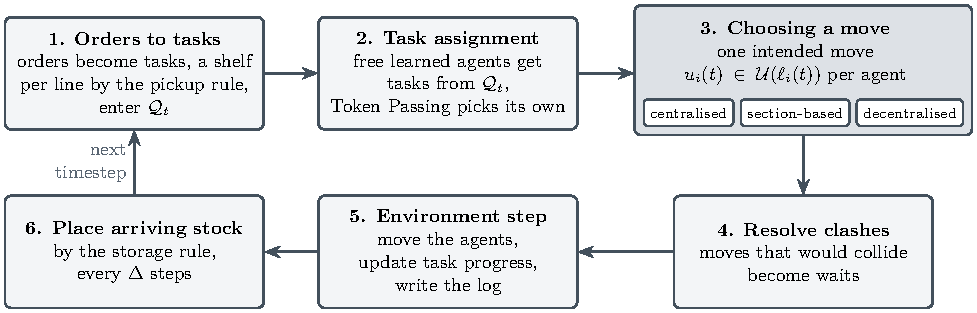
\includegraphics[width=\linewidth]{method_storage_fig/methodloop_proposed_v2.pdf}
\end{center}
\note{Greys only. Words follow the text, ``swaps with the controller'' goes,
stage 6 says ``every $\Delta$ steps'' instead of a dashed border. Source
\texttt{method\_storage\_fig/methodloop\_proposed\_v2.tex}. It replaces
\texttt{scripts/images/methodloop.tex} and \texttt{thesis/Images/methodloop.pdf}
when the section is applied.}

\section*{Part 3. Where arriving stock goes}

\old{The three storage rules form a ladder, and each rung adds one kind of
information. Fixed storage sends every SKU to its own home shelf. Demand
storage puts the SKUs ordered most often on the shelves with the shortest
trip. Congestion-aware storage does the same, but it avoids shelves where
picks often stand still, and it also picks from them less. The gap between
the last two shows what reading the time agents stand still adds to demand
alone, which is the storage half of RQ2.} \note{Third telling of the rules.
The gap between demand and congestion-aware storage is said in the Problem
Formulation, ``Under congestion-aware storage''. Start with the rule.}

\old{All three rules place arriving stock the same way, and only their order
differs. They take one SKU at a time. Its arriving units \nref{eq:arrivals}
come on pallets of $Q$, and each pallet goes whole onto the first shelf in
the rule's order with room for it under \eqref{eq:feasiblestorage}. A
pallet that fits nowhere is not placed. Stock already on a shelf stays
where it is (Section~\ref{sec:pf:storage}).}
\new{Every rule takes one SKU at a time and places it the same way. Only the
ranking differs, the order in which a rule takes the SKUs and, for each SKU,
the order of its shelves. A SKU's arriving units~\eqref{eq:arrivals} come on
pallets of $Q$. Each pallet goes whole onto the first shelf in the ranking
with room for it under~\eqref{eq:feasiblestorage}. A pallet that fits on no
shelf is lost (Section~\ref{sec:pf:storage}).} \note{``Order'' becomes
``ranking'', since the reader has customer orders in mind. ``Stock stays''
is in the Problem Formulation.}

A shelf is judged by the trip a unit makes through it, \dots\ \note{the
trip paragraph, the two legs, their weights and the tea example are
unchanged} \dots\ so tea goes to $A$, closer to its workstations, because it
is picked far more often than it is put away.
The demand rules are not told a SKU's category $h(k)$\new{, because they
read only the orders (Section~\ref{sec:pf:storage})}. They learn it from its
first order line, which always goes to a workstation of that category.
\new{A SKU gets its first pallet only after $Q$ of its units are ordered, so
its category is always known by then.} Fixed storage uses $h(k)$ directly.

The demand rules can be read as keeping a cost small. The classic slotting
cost $D$ adds up, over the pallets placed at an update, how often their SKU
is picked times the second leg, plus how often it gets a pallet times the
first leg. The blocking cost $K$ is the thesis's own\old{, because the
classic problem has no traffic}. It adds up, over the same pallets, how
often their SKU is ordered times how long picks stand still at their shelf.
Every pick from that shelf meets the wait, so a popular SKU pays it more
often. Formally, write $x^{\mathrm{new}}_t(k,v)$ for the units of SKU $k$
placed on shelf $v$ at this update. The two costs \old{and the value the
rules aim to keep small} are
\begin{equation*}
\begin{aligned}
D &= \sum_{k\in\mathcal{K}}\sum_{v\in V_{\mathrm{str}}}
  \bigl(\hat\rho_t(k)\,d^{\mathrm{work}}(k,v)+\hat\rho^{\mathrm{pal}}_t(k)\,d^{\mathrm{dock}}(v)\bigr)\,x^{\mathrm{new}}_t(k,v),
\\
K &= \sum_{k\in\mathcal{K}}\sum_{v\in V_{\mathrm{str}}}
  \hat\rho_t(k)\,\hat\omega_t(v)\,x^{\mathrm{new}}_t(k,v)\old{,
  \qquad D+\beta K} .
\end{aligned}
\tag{\lab{eq:storageobjective}}
\end{equation*}
\new{The rules aim to keep $D+\beta K$ small. Here $\beta \ge 0$ weights
standing still against travel distance, and its value is set in
Appendix~\ref{app:cal:beta}. The demand estimate is counted per step, so
$\beta$ stays comparable across the sweep of the storage period $\Delta$.}
Demand storage has $\beta=0$. Neither rule searches for the smallest value.
This is a score for ranking shelves, not the objective of the thesis, which
is the order time of Section~\ref{sec:pf:measures}.
\note{The cost stays before the rules, so the display does not move. $\beta$
is now explained where it first appears. ``Greedy'' is said only here.}

\textbf{Fixed storage} ($F_{\mathrm{fix}}$) gives every SKU a home shelf
once, at the start, with the most popular SKUs on the shelves nearest the
workstations of their category\old{ (Section~\ref{sec:impl:instances})}.
\dots\ \note{rest unchanged. The reference pointed forward to the
Experiments chapter, and the sentence is complete without it.}

\textbf{Demand storage} ($F_{\mathrm{dem}}$) is the classic slotting rule
\citep{heskett1963coi,dekoster2007picking}, applied to arriving stock. It
takes the SKUs from most to least ordered, by the estimated demand
$\hat\rho_t(k)$, and gives each the shelves with the smallest weighted
legs. The weights differ per SKU, so each SKU has its own \old{order}
\new{ranking} of shelves. \old{This keeps the slotting cost $D$ of
\nref{eq:storageobjective} small, with $\beta=0$, greedily and not
exactly.}

\textbf{Congestion-aware storage} ($F_{\mathrm{cng}}$) adds standing still to
the trip. Take two shelves with the same weighted legs, one where picks
rarely stand still and one where they often do. Demand storage treats them
as equal, and congestion-aware storage prefers the quiet one. Formally, the
\emph{congestion-aware score} of SKU $k$ at shelf $v$ is
\begin{equation*}
  \mathrm{score}(k,v) = \hat\rho_t(k)\,\bigl(d^{\mathrm{work}}(k,v)
  + \beta\,\hat\omega_t(v)\bigr) + \hat\rho^{\mathrm{pal}}_t(k)\,d^{\mathrm{dock}}(v) .
  \tag{\lab{eq:storagegreedy}}
\end{equation*}
\old{The weight $\beta \ge 0$ sets how much standing still counts against
distance (Appendix~\ref{app:cal:beta}).} Standing still joins the second
leg, because every pick from the shelf meets it. SKUs go from most to least
ordered, and each pallet goes to the shelf with the lowest score that has
room for it. \old{This keeps $D+\beta K$ of \nref{eq:storageobjective}
small, greedily and not exactly.}

\old{The demand estimate is the rate per step of \nref{eq:estimates} over
the last storage period. Counting per step keeps $\beta$ comparable across
the sweep of the storage period $\Delta$. If no order was released in a
period, nothing was picked and nothing arrives.} \note{The estimate is
already per step in the Problem Formulation. The reason moved up to the
$\beta$ sentence. The quiet-period sentence goes, since the Problem
Formulation's estimate already gives zero.}

\old{The time standing still comes from the picks that finished in the
period. For each, the steps its agent stood still while serving it are
counted, the blocked part of its service time \nref{eq:split}. The average
over a shelf's picks is that shelf's reading for the period. A shelf gets
only a few picks in one period, about eight at 8 agents, so one reading
alone jumps around. $\hat\omega_t(v)$ is therefore the plain average of the
shelf's last five readings. A shelf with no pick in a period keeps its
average, and a shelf with no reading yet counts zero.}
\new{A shelf's reading for one period is the mean steps stood still by the
picks from it that finished in the period, the blocked part of their
service time~\eqref{eq:split}. $\hat\omega_t(v)$ is the plain average of
the shelf's last five readings. Five is a practical smoothing choice. It
evens out one noisy period and still follows recent congestion, and the
number was not tuned. A shelf with no pick in a period keeps its average.}
Formally, write $\bar W_s(v)$ for the mean steps stood still by the picks
from $v$ that finished in period $s$, and $S_t(v)$ for the last five
periods in which $v$ had such a pick. Then
\begin{equation*}
  \hat\omega_t(v) = \frac{1}{|S_t(v)|}\sum_{s \in S_t(v)} \bar W_s(v) .
  \tag{\lab{eq:standstill}}
\end{equation*}
\note{Few picks, jumping readings and ``no pick yet reads 0'' are in the
Problem Formulation's ``What the rule reads''. ``About eight at 8 agents''
goes with them. The two symbols stay, because the formula needs the set of
periods.}

\old{Under congestion-aware storage the pickup rule also adds
$\hat\omega_t(v)$ to each shelf's distance (Section~\ref{sec:pf:tasks},
Orders and tasks), and the other rules keep the nearest shelf. When two
shelves are equally near, the one with the lower vertex number goes first.}
\note{The Problem Formulation's pickup paragraph says it. The tie joins
the ties below.}

\old{Placing arriving stock was chosen over relocating stored stock, because
it changes the layout more without assuming that moving stock is free. A
pilot with Token Passing supports the choice
(Appendix~\ref{app:cal:arrival}).} \note{Moves to the Problem Formulation,
where ``stock already on a shelf stays'' is set, see Part~5.}

\old{Ties between SKUs are broken by index. Ties between shelves are broken
by the plain trip of the shelf~\eqref{eq:shelftrip} and then by index, so
each rule gives exactly one placement (Appendix~\ref{app:storage:ties}).}
\new{Ties between SKUs go by index. Ties between shelves go by vertex index,
both when stock is placed and when a line picks. When stock is placed, the
plain trip of the shelf~\eqref{eq:shelftrip} is compared first. So each rule
gives exactly one placement (Appendix~\ref{app:storage:ties}).}
\old{The arrivals are the same under every rule, because they depend only on
the orders.} \note{Said in the Problem Formulation, ``How stock changes''.}
The storage period, the congestion weight and the other storage values are
set in Appendix~\ref{app:storagecal}.

\section*{Part 4. Who takes which task}
\old{Every learned controller uses the same assignment rule, so a difference
in results never comes from assignment.} \note{Third telling, the Problem
Formulation says it.}
\new{Task assignment is held fixed on purpose. The thesis studies how
storage and the choice of moves affect each other, so a better assignment
rule is out of scope, and every learned controller uses the same simple
one.} Each waiting task, oldest first, goes to the nearest free agent\new{,
counted from the agent to where the task picks up, the shelf of a pick or
the dock of a put-away}. \old{, and that} \new{That} agent is then no
longer free. Formally, the \emph{assignment rule} gives task $\tau_j$ to
\begin{equation*}
  i^\star(j) = \arg\min_{i \,:\, a_i \text{ free}} d_G(\ell_i(t), s_j) .
  \tag{\lab{eq:assignmentrule}}
\end{equation*}
\new{Take a pick of tea from shelf $A$ of Table~\ref{tab:storagematrix} and
two free agents, $a_1$ three steps from $A$ and $a_2$ five steps. The task
goes to $a_1$. Had both been three steps away, the priority order below
would decide.}

Picks and put-aways wait in the same queue and are taken alike. A put-away
gets no priority of its own, because oldest first is the simplest rule and
adds no parameter. \new{A put-away that waits keeps its units from being
picked, so at a high load a priority for put-aways might shorten the wait
for stock. The Discussion returns to this.} Tasks released in the same
timestep go in order of task index. Between two free agents at the same
distance, the priority order of Section~\ref{sec:pf:controllers} decides.
That order is drawn again each episode, so no agent is always favoured. The
rule is simple and not optimal. An optimal matching could replace it without
changing anything else. \old{Token Passing chooses its own tasks
(Section~\ref{sec:method:reference}).} \note{Now in the loop at the start.}

\section*{Part 5. The Problem Formulation}
Line numbers are of \texttt{3.ProblemFormulation.tex} today.

\textbf{5.1 Arrival-only placement, its reason (line 304, ``The storage
rule'').} A storage rule decides where arriving stock goes, and nothing
else. Stock already on a shelf stays where it is until it is picked.
\new{This was chosen over also moving stored stock, because every arriving
pallet is a new choice of shelf that needs no extra trip. Moving stored
stock would need trips of its own, or would have to assume they cost
nothing. A pilot with Token Passing supports the choice. Demand storage
that placed arriving stock cut service time by about 43\% against fixed
storage, and moving up to a fixed number of stored units per period by
25\% (Appendix~\ref{app:cal:arrival}).} This is the dynamic storage
location assignment problem \dots

\textbf{5.2 Fixed storage overflow (line 310 and Table \lab{tab:rules}).}
\dots\ sends each pallet back there, whatever the orders say. \new{A pallet
that does not fit at home goes to the nearest shelf with room.} This is the
dedicated storage \dots\ \note{40 to 60\% of arriving units under the
learned controllers, 8\% under Token Passing, from
\texttt{review\_trip\_legs}.} In the table, fixed, where new stock goes:
the SKU's home shelf\new{, or the nearest shelf with room}.

\textbf{5.3 ``The rules are greedy'' (line 325).} \old{The rules are greedy.
They place one SKU at a time on its best shelf with room, and none of them
claims to find the best possible placement.} \note{How a rule searches is
method. The Method says it once.}

\textbf{5.4 A lost pallet (line 384, the storage update).} \dots\ a pallet
that fits on no shelf is left unplaced. \new{An unplaced pallet is lost. Its
units do not count towards the SKU's next pallet, so a line that waited for
them waits for a later one.} A storage rule is any $F$ \dots

\textbf{5.5 One name for the storage update.} ``Storage epoch'' becomes
``storage update'' in both notation tables (\texttt{2.Notation.tex} line 83,
\texttt{A.Notation.tex} line 85, ``at each storage \old{epoch}
\new{update}'') and in the Experiments mock-up (line 225, ``many storage
\old{epochs $\Delta$} \new{periods}''). ``Storage period'' stays for the
$\Delta$ steps between two updates, as the Problem Formulation defines it.
The commented-out lines in the Problem Formulation are left alone.

\textbf{No change needed.} ``The thesis's own, because the classic problem
has no traffic'' (line 322) is now said only here. ``The gap between demand
and congestion-aware storage shows only what reading congestion adds''
(line 738) and ``a shelf with no pick yet reads 0'' (line 365) stay, and
the Method's versions go.

\section*{Part 6. Controllers and conflict resolution}
The comments PDF has five green sentences here. Each is checked against
what the text already says.
\begin{enumerate}[label=\alph*)]
  \item \emph{``\dots never overrides a centralised agent, and the override
    term of the reward is always zero for it.''} \textbf{Leave out.} The
    reward section already says ``A centralised agent never pays it''
    (\texttt{4.Implementation.tex} line 633).
  \item \emph{``The halo uses the same range as the field of view, so the
    crowding feature means the same under every controller.''}
    \textbf{Merge.} The text says the halo is as wide as the field of view
    twice (lines 428 and 434). Keep the first and give the reason once:
    \old{The halo reaches as far as the field of view, so the window of an
    agent at the zone edge still holds its whole field of view.} \new{So an
    agent at the zone edge still sees its whole field of view, and its
    features, crowding among them, mean the same as under the other
    controllers.}
  \item \emph{``With $p=1$ the halo is empty and the section-based controller
    is the centralised one.''} \textbf{Add}, after ``Conflict resolution
    removes these clashes as it does everywhere else.'' It follows from the
    definitions, one zone covers the whole warehouse, and it helps the
    reader place the two controllers.
  \item \emph{``The three learned controllers share the network, the masks,
    the reward and the training \dots''} \textbf{Leave out.} The Problem
    Formulation's ``What the controllers share'' says it, and the comment
    on the opening asks to say it once.
  \item \emph{``Token Passing plans ahead and does not meet this circle.''}
    \textbf{Add, as a pointer}: \new{Token Passing never meets this circle
    (Section~\ref{sec:method:reference}).} The reason is given there.
\end{enumerate}

\section*{Part 7. Every comment and where it is handled}
\small
\begin{longtable}{p{0.55\linewidth}p{0.38\linewidth}}
\toprule
comment & handled \\
\midrule
\multicolumn{2}{l}{\emph{First set (pasted)}} \\
1. Token Passing in loop step 2 & Part 2, loop prose \\
2. List and Figure 12 duplicate, labels, caption & Part 2, list goes, figure v2 \\
3. Ladder, ``storage half of RQ2'', greedy once & Part 3, first paragraph struck, greedy once \\
4. $\beta$ before it is explained & Part 3, sentence after the display \\
5. Lost pallet, category before first line & Parts 1, 3 and 5.4 \\
6. $K$ reason once, pickup paragraph, ties & Parts 3 and 5 \\
7. Arrival-only reason, split last paragraph & Part 5.1, ties and values in Part 3 \\
8. Five readings & Part 3 \\
9. Floating sentence & Part 3, struck \\
10. Code check, references & Part 1, labels unchanged \\
\midrule
\multicolumn{2}{l}{\emph{Second set (\texttt{method\_assignment\_comments.pdf})}} \\
Opening says what the PF says & Part 2, struck \\
Sentence about the text & Part 2, struck \\
Token Passing exception later & Part 2 \\
epoch, update, period & Part 5.5 \\
\texttt{\textbackslash nref} doubles & Parts 2 and 3, now \texttt{\textbackslash eqref} \\
Do the subsections follow the loop & Part 2, storage first, with the reason \\
Figure 12 words, caption name & Part 2 \\
Storage half of RQ2, ladder, ``order'' & Part 3, ``ranking'' \\
Lost pallet, stock stays repeats & Parts 3 and 5.4 \\
Legs not weighted, overflow order, ``as often as picked'' & already fixed [A122] \\
Why $h(k)$ is estimated & Part 3, one clause \\
$D+\beta K$ alone in the display & Part 3, moved into the sentence \\
Broken VIII-A0c, forward ref & fixed [A109], forward ref struck \\
Greedy said three times & Parts 3 and 5.3 \\
Estimate repeats PF & Part 3 \\
Standing still repeats PF, ``about eight'', two symbols & Part 3 \\
Pickup paragraph, ties twice & Part 3 \\
Arrival-only reason at the end, ``more'' than what & Part 5.1 \\
Third telling, start with the rule & Part 3 \\
Why oldest first and nearest, source & Part 4, question 3 \\
Nearest to what & Part 4 \\
Worked example & Part 4, tea on shelf $A$ \\
Put-away priority & Part 4, question 4 \\
Assignment out of scope & Part 4 \\
Token Passing line at the end & Part 4, struck \\
Five green sentences & Part 6 \\
\bottomrule
\end{longtable}
\normalsize

\section*{Questions}
\begin{enumerate}
  \item \textbf{Lost pallets break the Appendix E rule.} Appendix E requires
    zero failed placements at the main load and drops a setting that has
    many. Token Passing meets it, but the long decentralised run under
    fixed storage loses 15\% of arriving units, and several arms 2 to 4\%.
    This is a result to note. I propose a column in the Appendix L table,
    one sentence in the Results, and a change to Appendix E's rule so it
    says it was checked with Token Passing and that learned arms are
    reported, not dropped. Agree?
  \item \textbf{Pilot numbers.} You said keep them in the Method. With the
    reason moved to the Problem Formulation (5.1), they go with it. Fine, or
    keep a pointer in the Method too?
  \item \textbf{Where the assignment rule comes from.} Neither the code nor
    GAPS names a source. Ma et al.\ (2017) is not it, since there each agent
    takes a task itself. I wrote it as the thesis's own simple rule. Do you
    have a source in mind?
  \item \textbf{Put-away priority.} The new sentence promises the Discussion
    returns to it. Should it, or drop that sentence?
  \item \textbf{The example on Table I.} Table~I is the storage state, so the
    example uses tea on shelf $A$ from it, with made-up agent distances.
    Fine?
\end{enumerate}

\end{document}
